
\chapter{知识协同动机因素模型仿真与决策分析}
\label{cha:emulation}

在上一章中,本文提出了个体参与社区知识协同的动机因素模型,描述了动机因
素与协同行为的关系。为了进一步验证模型的有效性,以及利用模型分析社区中
知识协同行为的演化过程,为管理决策提供依据,需要对模型进行仿真实验。

\section{动机因素模型仿真}

\subsection{仿真的基本过程}
建立模型要素的因果回路是模型仿真的第一步。但是仅靠因果回路图是无法进行
仿真的。因果回路图的适用范围是表达系统要素间的关联和反馈过程,但是变量
的性质却未能因果回路图中并没有表现出来。因果回路图无法描述系统管理和控
制过程,因此被应用于早期建模过程中,重点反应最基本的模型结构,方便建模
者对模型主体的把握。

流量和存量是社会经济系统中的两种基本变量。存量反映了系统在某一时刻的状
态,而流量则揭示了存量的变化快慢情况,这在因果图中是无法体现出来的。存
量变化的速率是系统演化的重要决定因素之一。因此,区分存量和流量是对因果
关系更细致和深入的描述,反应系统中各要素的控制与反馈。在存量流量模型的
基础上,通过设定各个变量的初值,步长等参数,用方程来描述各因素间的函数关
系,最终得到系统仿真的模型。通过多次试运行和调整,以及对模型进行有效性
检验,使模型可以较准确地反映现实世
界的变动,研究者可以利用模型进行决策分析。模型仿真的基本过程如图\ref{fig:vensim}所示。
\begin{figure}[htb]
  \centering
  \scalebox{0.7}{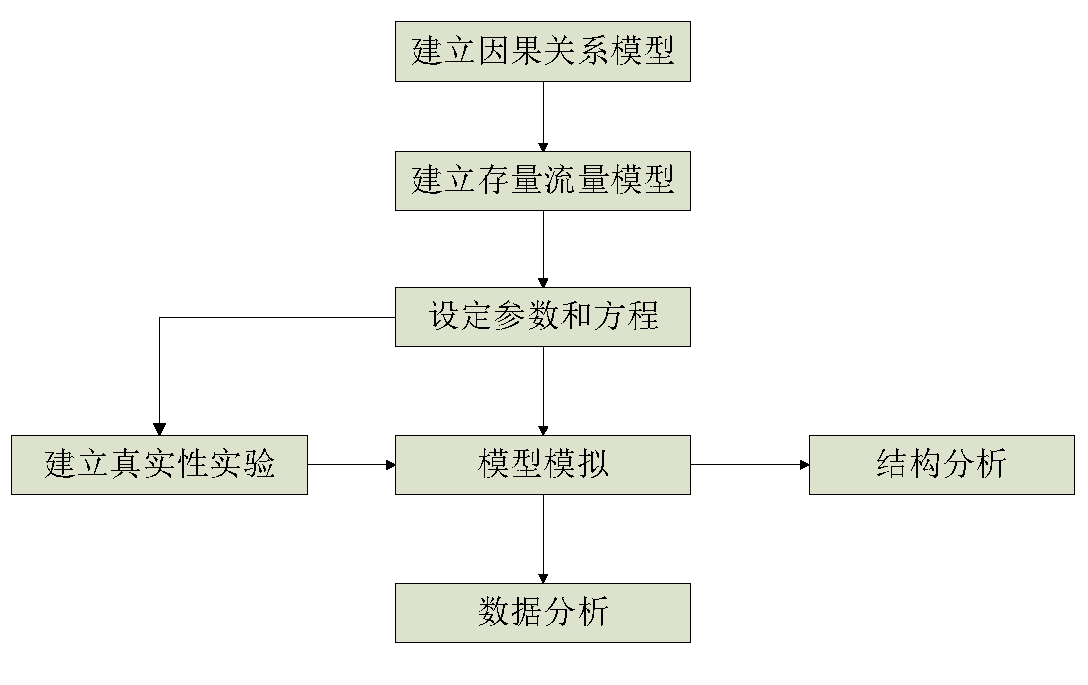
\includegraphics{vensim.pdf}}
  \caption{模型仿真过程}
  \label{fig:vensim}
\end{figure}
\subsection{动机因素存量流量图}

在因果图中,不论是动机因素,还是个体的行为都是系统的状态,是存量。为了
描述动机于行为间的关系而故意忽略了一些流量变量和外生变量。但是,这些被
忽略的变量对于整个系统起到了重要作用,没有这些变量系统就不可能正确地表
示现实系统的运行。

对于大部分动机因素,它们和个体的行为之间构成了一个正反馈回路和一个负反
馈回路,既动机的
增强会提升个体的行为水平,如果协同行为的得到了他人的正反馈,则会提升个体的动
机;反之如果协同行为得到了他人的负反馈,个体的动机会受到伤害。对于现实
系统来说,有几个重要的变量未能包含在因果图中。首先,个体的协同行为水平
不仅受到动机的影响,还受到其他因素,尤其是个体工作能力的限制。无论个体怎么
提升协同水平,都不可能超过个体的最大工作能力。这就是所谓“增长的极限”。
个体的最大工作能力是行为水平的抑制因素,使得行为水平不可能无限制地增长
下去。其次,动机作为系统中的存量,必然要受到流量的影响。动机的流
入是从协同活动中获得的正反馈转化的动机,动机的流出则是协同活动中获得的
负反馈使动机削弱的数量。流入水平和流出水平综合决定了动机存量的变化。第
三,不论是动机转化为行为还是行为的结果反馈影响动机都不是线性过程。这种
变换也存在遍及递减效应,动机的水平越高,每增加一单位动机所能引起的行为
水平的增加就越少。因此如果仅考虑行为与动机的互动关系的话,个体的动机应
该呈对数增长(或减弱),最后接近某个极大(小)值。最后,成就动机同其他
动机略有不同。成就动机促使个体参与某种活动从中获得成就感。成就感的提升
削弱成就需求。但是成就感有一种随时间自动削弱的属性,在没有任何外力介入
的情况下成就感将逐渐流失,从而提升了个体的成就需求,促使他们参与新的活
动重新获得成就感。流失速度的不同决定了不同人的行为模式,对于流失速度快
的人来说,他们从参与活动中所获得的成就感迅速减少,因此这些人表现为进取
精神非常强,不停地追逐新的目标来满足自己对成功的渴望。而流失速度慢的人则
会很长时间满足于自身取得的成就,表现为为止步不前,不愿接受新的挑战。

根据以上分析的结果,本文将把因果关系图转换为存量流量图,同时在模型中加
入新的变量,使模型更符合现实世界。因为转换的模型力图完整描述存量于流量
的关系,因此对因果关系进行了简化处理。变量间具体、详细的因果关系请参考
因果关系图。大部分的动机因素都有同样的特征:动机增加引起行为水平的提升;
如果行为得到正反馈则会促使动机也得到相应的提升,负反馈则会使动机减弱。
因此将这一类动机合并表示一般动机。对于利他主义和感知到的意义两类动机由
于和行为之间是单向关系,统称为无反馈动机。成就动机和认知失调两类动机有
各自的特点,所以单独保留。引入了流量变量“每次协同行为增加的动机”表示
动机的流入,“他人对个体的协同行为减少的动机”表示动机的流出,以此表示
动机的动态性;引入变量“疲劳“和外生变量“个人工作的最大能力”构建行为
的负反馈闭环,反应行为水平受到抑制的特征。引入流量变量“满足感的流失”
反应满足感随时间减少的特点。转换的存量流量图如图
\ref{fig:refined-model}所示。
\begin{figure}[htb]
  \centering
  \scalebox{0.7}{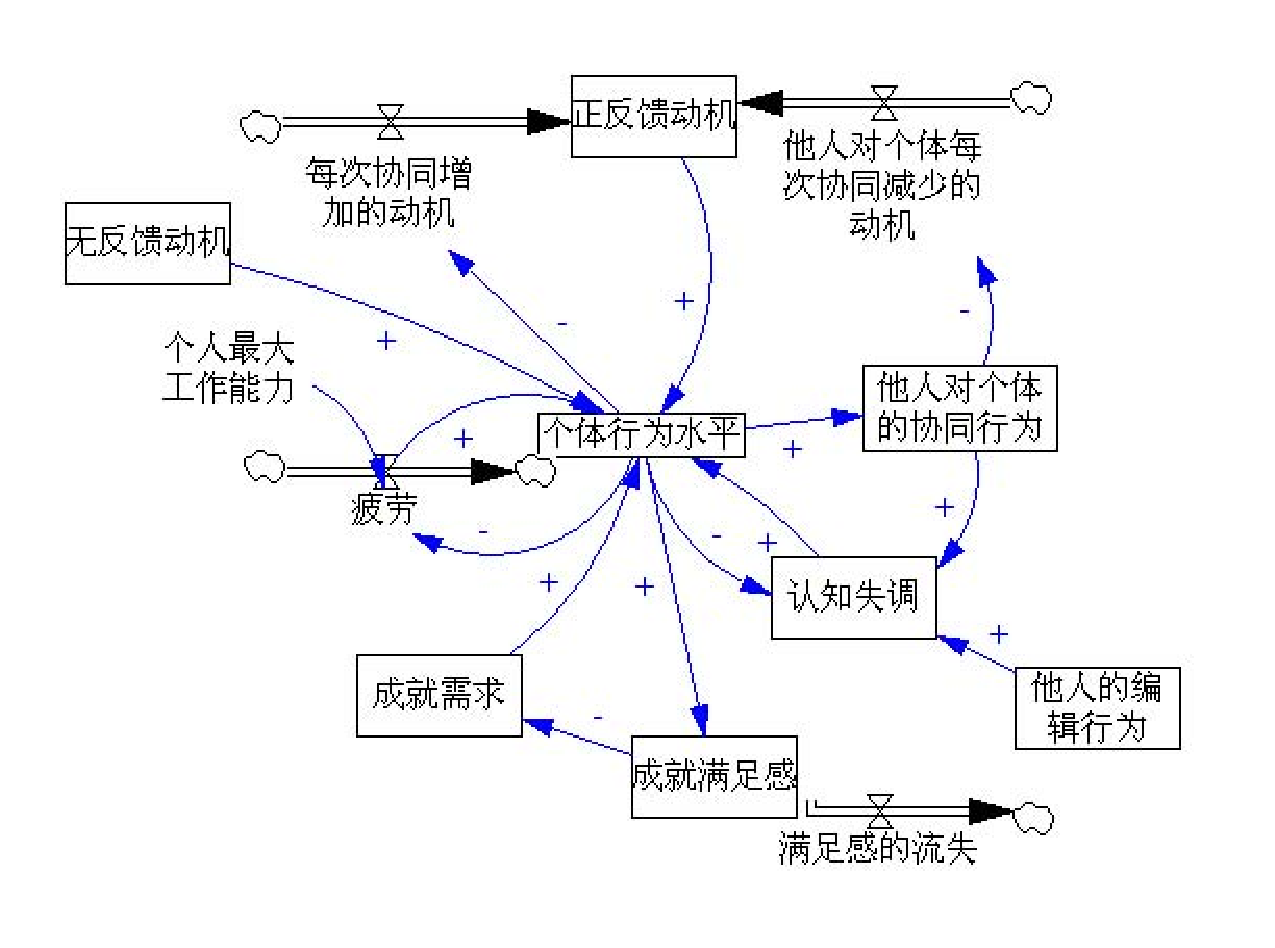
\includegraphics{refinedmodel1.pdf}}
  \caption{\small{知识协同动机因素的存量流量图}}
  \label{fig:refined-model}
\end{figure}

\subsection{模型方程的设置}

每个变量都和其他变量形成一定的函数关系,这种关系使用方程来表示。下面列
举了了模型中所有涉及到的方程。
\begin{enumerate}
\item 行为水平=转换水平$\times (\sum$一般动机+成就动机+认知失调+无反馈
  动机)
\item 成就需求=个体的最大成就需求-满足感$\times$转换系数
\item 认知失调=他人的协同行为$\times$转换系数+他人对个体的协同行为
  $\times$转换系数-协同行为水平$\times$转换系数
\end{enumerate}

%%% Local Variables: 
%%% mode: latex
%%% TeX-master: t
%%% End: 
